\section{基于增量舒尔补的优化方法}

iSAM2算法\cite{kaess2008isam,kaess2012isam2}创新性地在SLAM问题中使用了贝叶斯树来编码集束优化过程中的信息矩阵分解过程,达到高效地更新平方根信息矩阵的目的,显著地提升了全局优化的性能。其算法不仅适用于SLAM中的集束优化问题,也适用于一般的非线性最小二乘问题。也正是为了保证通用性,iSAM2难以在状态之间的关联特点高度统一的SLAM问题中发挥更高的性能。

例如在图\ref{fig:sparse_matrix}中,正规方程的三维点部分(左上角部分)高度稀疏,呈对角块状,在求解时应该优先考虑这一部分的分解。iSAM2算法需要依赖COLAMD\citep{davis2004algorithm}算法来被动地检测矩阵分解的顺序,一方面需要额外的计算时间,另一方面也不一定能得到比经验更好的结果。

\subsection{舒尔补}

舒尔补(Schur complement)是一种常用的加速求解稀疏线性系统的方法,也特别适用于集束优化问题中的正规方程的求解。其本质上是基于高斯消元的分块求解线性系统的方法。如下是一个集束优化问题中常见的正规方程的形式,其中$\mathrm{P}$是三维点状态对应的信息矩阵,$\mathrm{C}$是相机状态对应的信息矩阵,$\mathrm{W}$是三维点状态和相机状态的信息矩阵:
\begin{equation}
    \begin{bmatrix}
        \mathrm{P} & \mathrm{W}^\top \\
        \mathrm{W} & \mathrm{C}
    \end{bmatrix}
    \begin{bmatrix} \bm{\delta}_p \\ \bm{\delta}_c \end{bmatrix} =
    \begin{bmatrix} \bm{b}_p      \\ \bm{b}_c      \end{bmatrix}
\end{equation}
求解三维点状态和相机状态之前,先通过行变换构建舒尔补方程:
\begin{equation}
    \begin{bmatrix}
        \mathrm{P} & \mathrm{W}^\top \\
                 0 & \mathrm{C}-\mathrm{W}\mathrm{P}^{-1}\mathrm{W}^\top
    \end{bmatrix}
    \begin{bmatrix} \bm{\delta}_p \\ \bm{\delta}_c \end{bmatrix} =
    \begin{bmatrix}
        \bm{b}_p \\
        \bm{b}_c-\mathrm{W}\mathrm{P}^{-1}\bm{b}_p
    \end{bmatrix}
\end{equation}
其中$\mathrm{C}-\mathrm{W}\mathrm{P}^{-1}\mathrm{W}^\top$称为舒尔补。根据经验,集束优化问题中的三维点状态数量远多于相机状态数量,故矩阵$\mathrm{P}$的规模远大于舒尔补矩阵。通过求解下式
\begin{equation}
    \bm{\delta}_c = 
    \left( \mathrm{C}-\mathrm{W}\mathrm{P}^{-1}\mathrm{W}^\top \right)
    \enspace\setminus\enspace
    \left( \bm{b}_c-\mathrm{W}\mathrm{P}^{-1}\bm{b}_p \right)
    \label{eq:solve_schur}
\end{equation}
可以快速得到相机状态变量的值。又因为三维点之间没有直接通过因子相连,故其信息矩阵$\mathrm{P}$呈对角块稀疏状,如图\ref{fig:sparse_matrix}所示。因此,$\mathrm{P}^{-1}$矩阵的计算往往非常快速。通过回代,又可以高效地求解剩余变量:
\begin{equation}
    \bm{\delta}_p = \mathrm{P}
    \enspace\setminus\enspace
    \left( \bm{b}_p-\mathrm{W}^\top\bm{b}_c \right)
    \label{eq:back_sub}
\end{equation}

对于如图\ref{fig:factor_graph}所示的因子图。

\begin{figure}[htb]
    \centering
    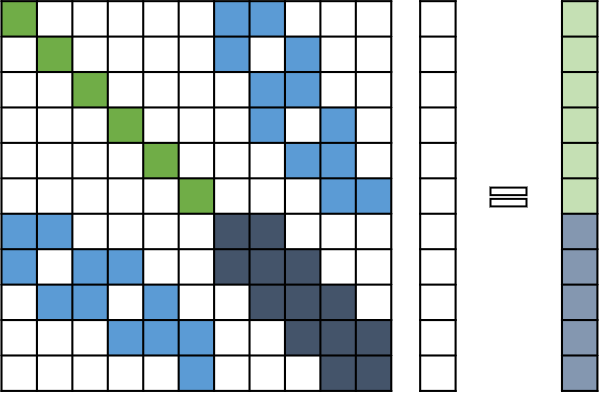
\includegraphics{figs/normal_eq.png}
    \caption{正规方程}
\end{figure}

\begin{figure}[htb]
    \centering
    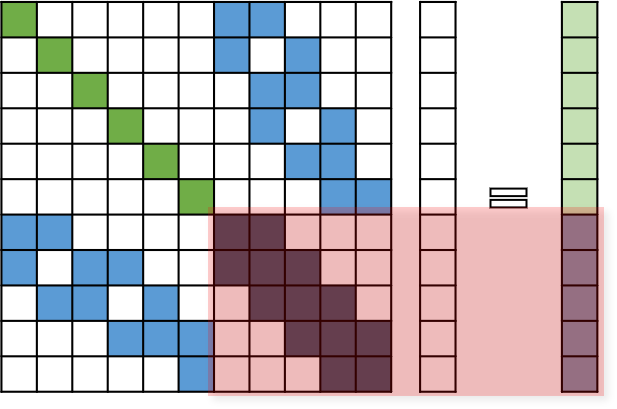
\includegraphics{figs/reduced_sys.png}
    \caption{舒尔补}
\end{figure}

\begin{figure}[htb]
    \centering
    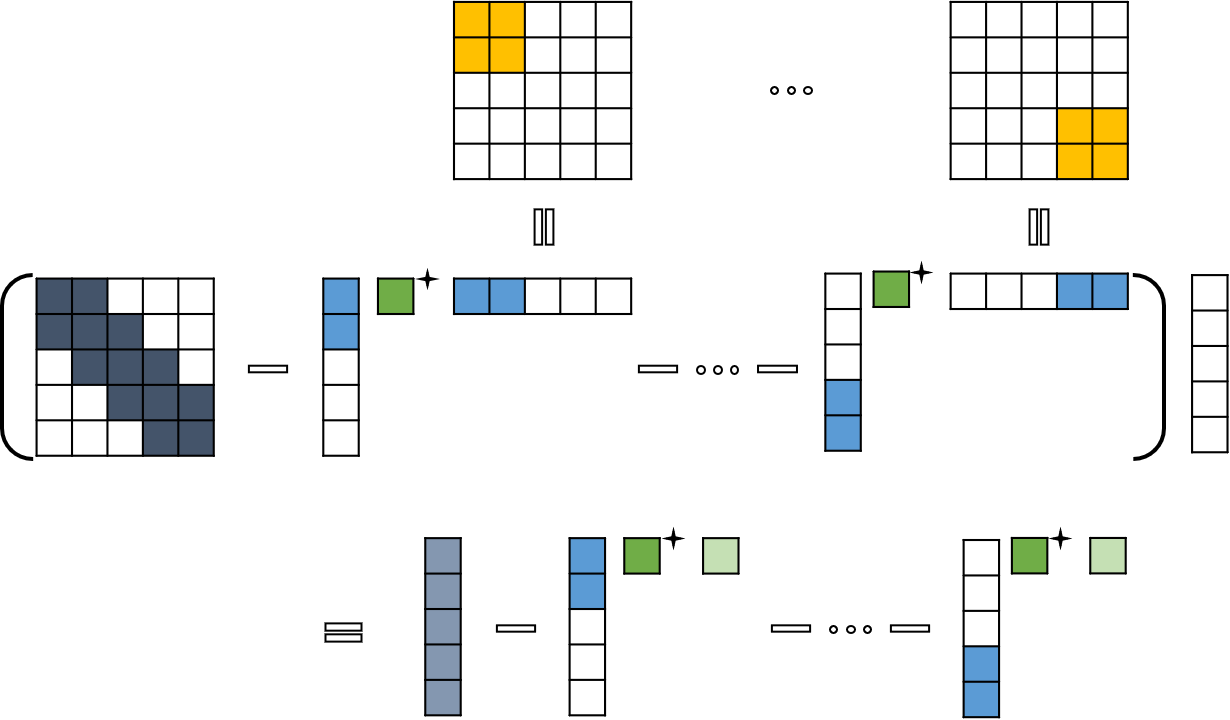
\includegraphics[width=\textwidth]{figs/schur_complement.png}
    \caption{计算舒尔补}
\end{figure}

\subsection{增量更新舒尔补}

\begin{figure}[htb]
    \centering
    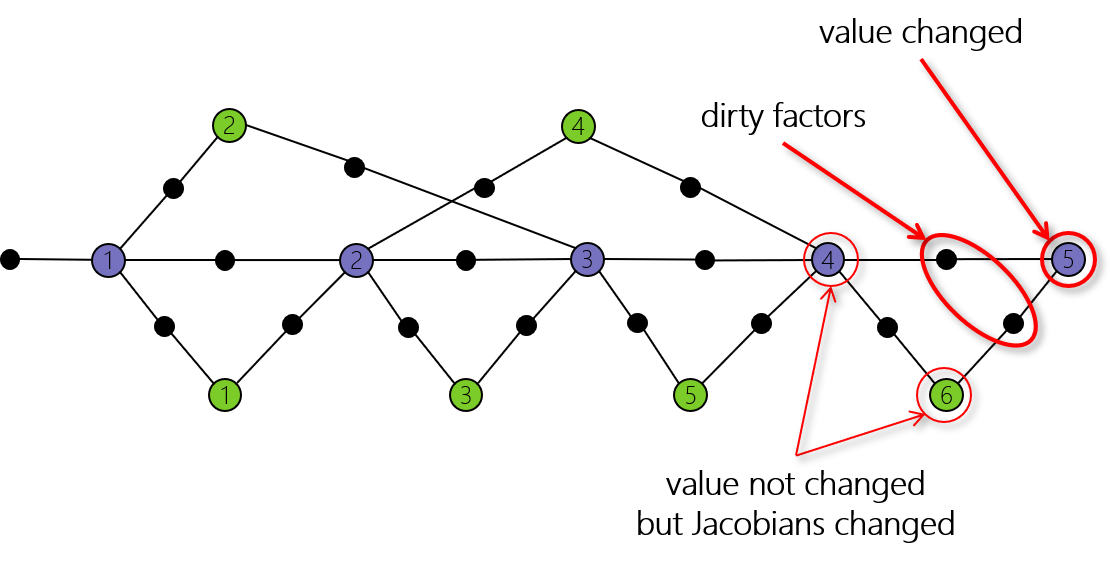
\includegraphics[width=\textwidth]{figs/factor_graph_dirty.png}
    \caption{标记因子图待更新部分}
\end{figure}

\begin{figure}[htb]
    \centering
    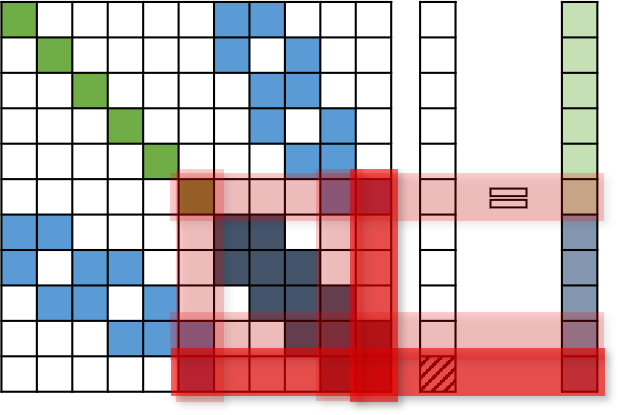
\includegraphics{figs/normal_eq_cursed.png}
    \caption{待更新舒尔补部分}
\end{figure}

\begin{figure}[htb]
    \centering
    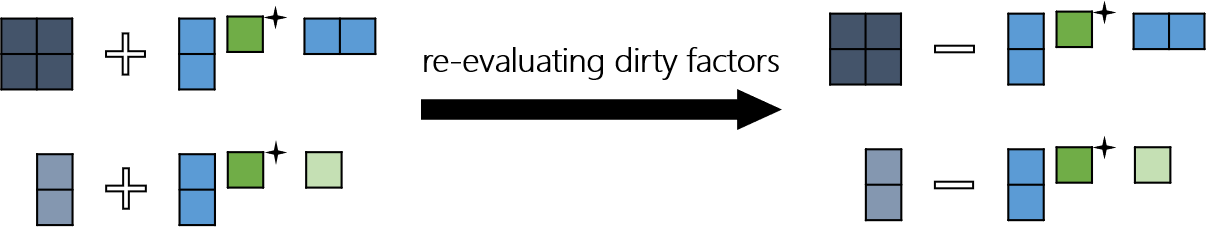
\includegraphics[width=\textwidth]{figs/schur_update.png}
    \caption{更新舒尔补}
\end{figure}

\subsection{状态增广}

\begin{figure}[htb]
    \centering
    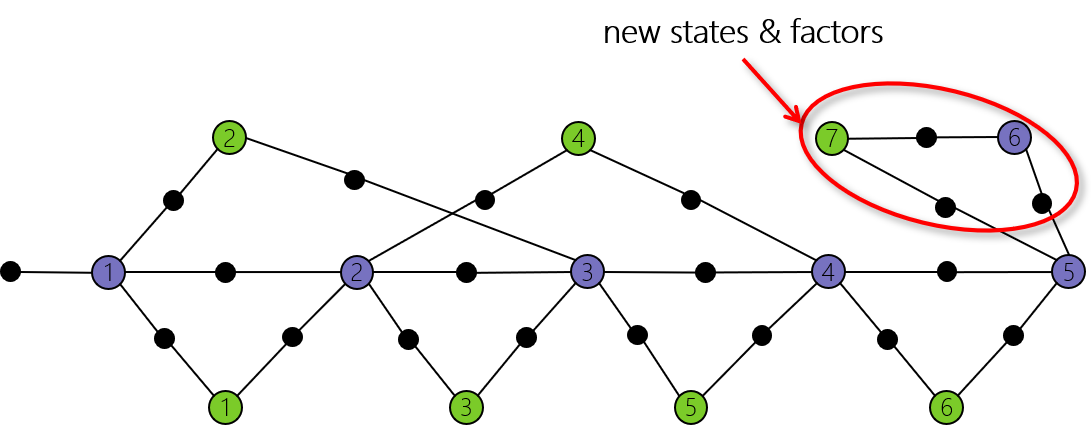
\includegraphics[width=\textwidth]{figs/factor_graph_aug.png}
    \caption{增广因子图}
\end{figure}

\begin{figure}[htb]
    \centering
    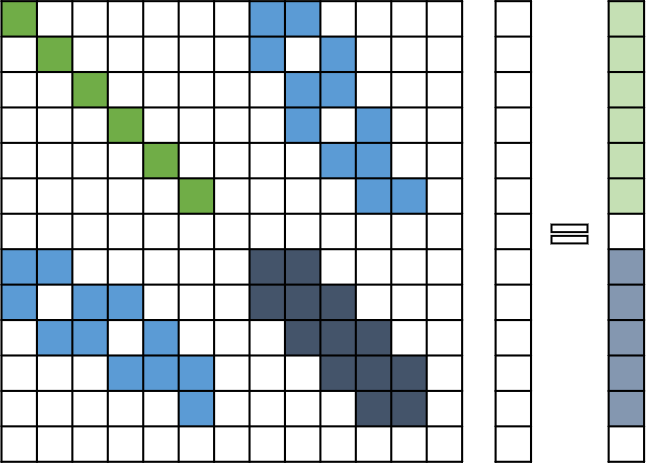
\includegraphics{figs/normal_eq_aug.png}
    \caption{增广正规方程}
\end{figure}

\begin{figure}[htb]
    \centering
    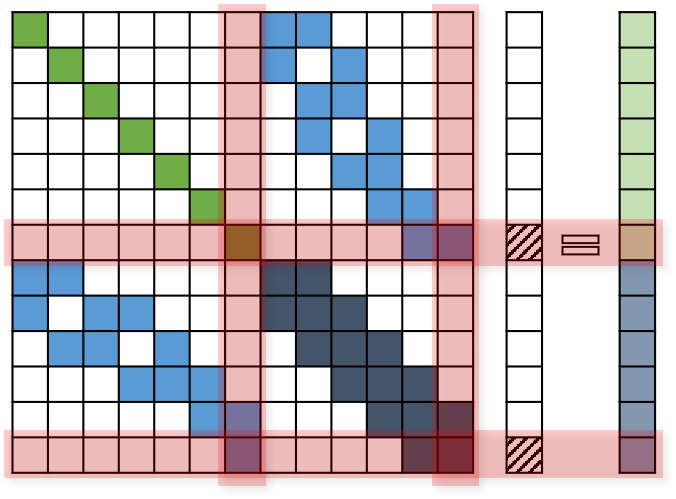
\includegraphics{figs/normal_eq_update.png}
    \caption{更新正规方程}
\end{figure}

\subsection{增量舒尔补方法和基于贝叶斯树的增量方法对比}

\begin{figure}[htb]
    \centering
    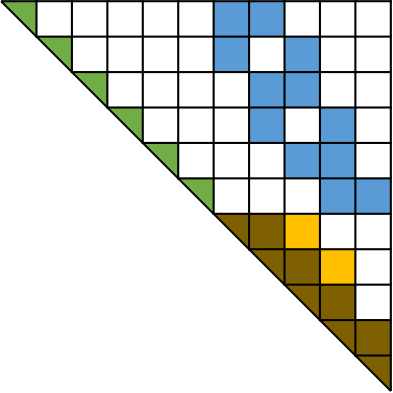
\includegraphics{figs/sqrt_info.png}
    \caption{平方根信息矩阵}
\end{figure}

\begin{figure}[htb]
    \centering
    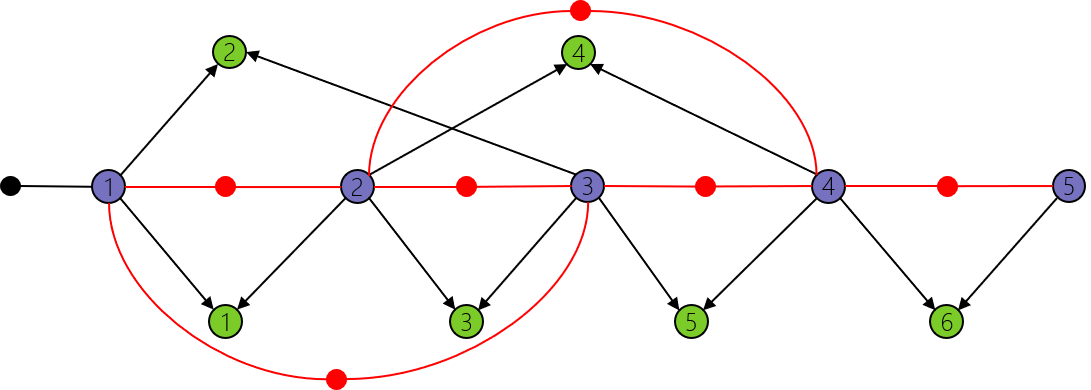
\includegraphics[width=\textwidth]{figs/elim.png}
    \caption{消元}
\end{figure}

\begin{figure}[htb]
    \centering
    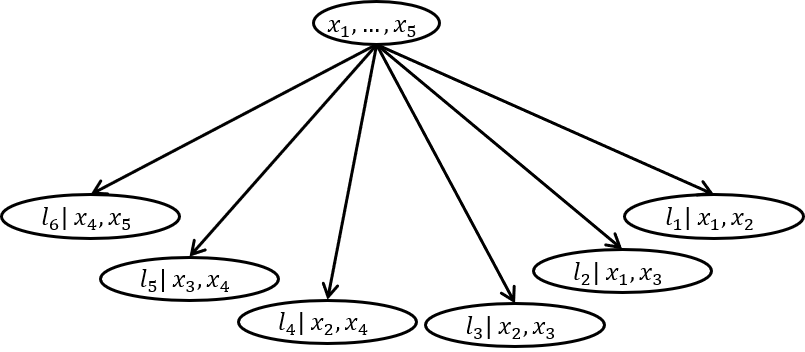
\includegraphics[width=\textwidth]{figs/bayes_tree.png}
    \caption{贝叶斯树}
\end{figure}
